%  LaTeX support: latex@mdpi.com
%  For support, please attach all files needed for compiling as well as the log file, and specify your operating system, LaTeX version, and LaTeX editor.

%=================================================================
% pandoc conditionals added to preserve backwards compatibility with previous versions of rticles
\documentclass[water,article,submit,oneauthor]{Definitions/mdpi}

% If you would like to post an early version of this manuscript as a preprint, you may use preprint as the journal and change 'submit' to 'accept'. The document class line would be, e.g., \documentclass[preprints,article,accept,moreauthors,pdftex]{mdpi}. This is especially recommended for submission to arXiv, where line numbers should be removed before posting. For preprints.org, the editorial staff will make this change immediately prior to posting.

%% Some pieces required from the pandoc template
\setlist[itemize]{leftmargin=*,labelsep=5.8mm}
\setlist[enumerate]{leftmargin=*,labelsep=4.9mm}


%--------------------
% Class Options:
%--------------------
%----------
% journal
%----------
% Choose between the following MDPI journals:
% acoustics, actuators, addictions, admsci, adolescents, aerobiology, aerospace, agriculture, agriengineering, agrochemicals, agronomy, ai, air, algorithms, allergies, alloys, analytica, analytics, anatomia, animals, antibiotics, antibodies, antioxidants, applbiosci, appliedchem, appliedmath, applmech, applmicrobiol, applnano, applsci, aquacj, architecture, arm, arthropoda, arts, asc, asi, astronomy, atmosphere, atoms, audiolres, automation, axioms, bacteria, batteries, bdcc, behavsci, beverages, biochem, bioengineering, biologics, biology, biomass, biomechanics, biomed, biomedicines, biomedinformatics, biomimetics, biomolecules, biophysica, biosensors, biotech, birds, bloods, blsf, brainsci, breath, buildings, businesses, cancers, carbon, cardiogenetics, catalysts, cells, ceramics, challenges, chemengineering, chemistry, chemosensors, chemproc, children, chips, cimb, civileng, cleantechnol, climate, clinpract, clockssleep, cmd, coasts, coatings, colloids, colorants, commodities, compounds, computation, computers, condensedmatter, conservation, constrmater, cosmetics, covid, crops, cryptography, crystals, csmf, ctn, curroncol, cyber, dairy, data, ddc, dentistry, dermato, dermatopathology, designs, devices, diabetology, diagnostics, dietetics, digital, disabilities, diseases, diversity, dna, drones, dynamics, earth, ebj, ecologies, econometrics, economies, education, ejihpe, electricity, electrochem, electronicmat, electronics, encyclopedia, endocrines, energies, eng, engproc, entomology, entropy, environments, environsciproc, epidemiologia, epigenomes, est, fermentation, fibers, fintech, fire, fishes, fluids, foods, forecasting, forensicsci, forests, foundations, fractalfract, fuels, future, futureinternet, futurepharmacol, futurephys, futuretransp, galaxies, games, gases, gastroent, gastrointestdisord, gels, genealogy, genes, geographies, geohazards, geomatics, geosciences, geotechnics, geriatrics, grasses, gucdd, hazardousmatters, healthcare, hearts, hemato, hematolrep, heritage, higheredu, highthroughput, histories, horticulturae, hospitals, humanities, humans, hydrobiology, hydrogen, hydrology, hygiene, idr, ijerph, ijfs, ijgi, ijms, ijns, ijpb, ijtm, ijtpp, ime, immuno, informatics, information, infrastructures, inorganics, insects, instruments, inventions, iot, j, jal, jcdd, jcm, jcp, jcs, jcto, jdb, jeta, jfb, jfmk, jimaging, jintelligence, jlpea, jmmp, jmp, jmse, jne, jnt, jof, joitmc, jor, journalmedia, jox, jpm, jrfm, jsan, jtaer, jvd, jzbg, kidneydial, kinasesphosphatases, knowledge, land, languages, laws, life, liquids, literature, livers, logics, logistics, lubricants, lymphatics, machines, macromol, magnetism, magnetochemistry, make, marinedrugs, materials, materproc, mathematics, mca, measurements, medicina, medicines, medsci, membranes, merits, metabolites, metals, meteorology, methane, metrology, micro, microarrays, microbiolres, micromachines, microorganisms, microplastics, minerals, mining, modelling, molbank, molecules, mps, msf, mti, muscles, nanoenergyadv, nanomanufacturing,\gdef\@continuouspages{yes}} nanomaterials, ncrna, ndt, network, neuroglia, neurolint, neurosci, nitrogen, notspecified, %%nri, nursrep, nutraceuticals, nutrients, obesities, oceans, ohbm, onco, %oncopathology, optics, oral, organics, organoids, osteology, oxygen, parasites, parasitologia, particles, pathogens, pathophysiology, pediatrrep, pharmaceuticals, pharmaceutics, pharmacoepidemiology,\gdef\@ISSN{2813-0618}\gdef\@continuous pharmacy, philosophies, photochem, photonics, phycology, physchem, physics, physiologia, plants, plasma, platforms, pollutants, polymers, polysaccharides, poultry, powders, preprints, proceedings, processes, prosthesis, proteomes, psf, psych, psychiatryint, psychoactives, publications, quantumrep, quaternary, qubs, radiation, reactions, receptors, recycling, regeneration, religions, remotesensing, reports, reprodmed, resources, rheumato, risks, robotics, ruminants, safety, sci, scipharm, sclerosis, seeds, sensors, separations, sexes, signals, sinusitis, skins, smartcities, sna, societies, socsci, software, soilsystems, solar, solids, spectroscj, sports, standards, stats, std, stresses, surfaces, surgeries, suschem, sustainability, symmetry, synbio, systems, targets, taxonomy, technologies, telecom, test, textiles, thalassrep, thermo, tomography, tourismhosp, toxics, toxins, transplantology, transportation, traumacare, traumas, tropicalmed, universe, urbansci, uro, vaccines, vehicles, venereology, vetsci, vibration, virtualworlds, viruses, vision, waste, water, wem, wevj, wind, women, world, youth, zoonoticdis
% For posting an early version of this manuscript as a preprint, you may use "preprints" as the journal. Changing "submit" to "accept" before posting will remove line numbers.

%---------
% article
%---------
% The default type of manuscript is "article", but can be replaced by:
% abstract, addendum, article, book, bookreview, briefreport, casereport, comment, commentary, communication, conferenceproceedings, correction, conferencereport, entry, expressionofconcern, extendedabstract, datadescriptor, editorial, essay, erratum, hypothesis, interestingimage, obituary, opinion, projectreport, reply, retraction, review, perspective, protocol, shortnote, studyprotocol, systematicreview, supfile, technicalnote, viewpoint, guidelines, registeredreport, tutorial
% supfile = supplementary materials

%----------
% submit
%----------
% The class option "submit" will be changed to "accept" by the Editorial Office when the paper is accepted. This will only make changes to the frontpage (e.g., the logo of the journal will get visible), the headings, and the copyright information. Also, line numbering will be removed. Journal info and pagination for accepted papers will also be assigned by the Editorial Office.

%------------------
% moreauthors
%------------------
% If there is only one author the class option oneauthor should be used. Otherwise use the class option moreauthors.

%---------
% pdftex
%---------
% The option pdftex is for use with pdfLaTeX. Remove "pdftex" for (1) compiling with LaTeX & dvi2pdf (if eps figures are used) or for (2) compiling with XeLaTeX.

%=================================================================
% MDPI internal commands - do not modify
\firstpage{1}
\makeatletter
\setcounter{page}{\@firstpage}
\makeatother
\pubvolume{1}
\issuenum{1}
\articlenumber{0}
\pubyear{2023}
\copyrightyear{2023}
%\externaleditor{Academic Editor: Firstname Lastname}
\datereceived{ }
\daterevised{ } % Comment out if no revised date
\dateaccepted{ }
\datepublished{ }
%\datecorrected{} % For corrected papers: "Corrected: XXX" date in the original paper.
%\dateretracted{} % For corrected papers: "Retracted: XXX" date in the original paper.
\hreflink{https://doi.org/} % If needed use \linebreak
%\doinum{}
%\pdfoutput=1 % Uncommented for upload to arXiv.org

%=================================================================
% Add packages and commands here. The following packages are loaded in our class file: fontenc, inputenc, calc, indentfirst, fancyhdr, graphicx, epstopdf, lastpage, ifthen, float, amsmath, amssymb, lineno, setspace, enumitem, mathpazo, booktabs, titlesec, etoolbox, tabto, xcolor, colortbl, soul, multirow, microtype, tikz, totcount, changepage, attrib, upgreek, array, tabularx, pbox, ragged2e, tocloft, marginnote, marginfix, enotez, amsthm, natbib, hyperref, cleveref, scrextend, url, geometry, newfloat, caption, draftwatermark, seqsplit
% cleveref: load \crefname definitions after \begin{document}

%=================================================================
% Please use the following mathematics environments: Theorem, Lemma, Corollary, Proposition, Characterization, Property, Problem, Example, ExamplesandDefinitions, Hypothesis, Remark, Definition, Notation, Assumption
%% For proofs, please use the proof environment (the amsthm package is loaded by the MDPI class).

%=================================================================
% Full title of the paper (Capitalized)
\Title{Assessing linkages between watershed nutrient loading and estuary
water quality in Lavaca Bay, Texas}

% MDPI internal command: Title for citation in the left column
\TitleCitation{Assessing linkages between watershed nutrient loading and
estuary water quality in Lavaca Bay, Texas}

% Author Orchid ID: enter ID or remove command
%\newcommand{\orcidauthorA}{0000-0000-0000-000X} % Add \orcidA{} behind the author's name
%\newcommand{\orcidauthorB}{0000-0000-0000-000X} % Add \orcidB{} behind the author's name


% Authors, for the paper (add full first names)
\Author{Michael
Schramm$^{1}$\href{https://orcid.org/0000-0003-1876-6592}
{\orcidicon}}


%\longauthorlist{yes}


% MDPI internal command: Authors, for metadata in PDF
\AuthorNames{Michael Schramm}

% MDPI internal command: Authors, for citation in the left column
%\AuthorCitation{Lastname, F.; Lastname, F.; Lastname, F.}
% If this is a Chicago style journal: Lastname, Firstname, Firstname Lastname, and Firstname Lastname.
\AuthorCitation{Schramm, M.}

% Affiliations / Addresses (Add [1] after \address if there is only one affiliation.)
\address{%
$^{1}$ \quad Texas A\&M AgriLife Research - Texas Water Resources
Institute 1001 Holleman Dr.~E. College Station, TX
77840-2118; \href{mailto:michael.schramm@ag.tamu.edu}{\nolinkurl{michael.schramm@ag.tamu.edu}}\\
}

% Contact information of the corresponding author
\corres{Correspondence: \href{mailto:michael.schramm@ag.tamu.edu}{\nolinkurl{michael.schramm@ag.tamu.edu}}}

% Current address and/or shared authorship








% The commands \thirdnote{} till \eighthnote{} are available for further notes

% Simple summary
\simplesumm{A Simple summary goes here.}

%\conference{} % An extended version of a conference paper

% Abstract (Do not insert blank lines, i.e. \\)
\abstract{A single paragraph of about 200 words maximum. For research
articles, abstracts should give a pertinent overview of the work. We
strongly encourage authors to use the following style of structured
abstracts, but without headings: 1) Background: Place the question
addressed in a broad context and highlight the purpose of the study; 2)
Methods: Describe briefly the main methods or treatments applied; 3)
Results: Summarize the article's main findings; and 4) Conclusion:
Indicate the main conclusions or interpretations. The abstract should be
an objective representation of the article, it must not contain results
which are not presented and substantiated in the main text and should
not exaggerate the main conclusions.}


% Keywords
\keyword{keyword 1; keyword 2; keyword 3 (list three to ten pertinent
keywords specific to the article, yet reasonably common within the
subject discipline.).}

% The fields PACS, MSC, and JEL may be left empty or commented out if not applicable
%\PACS{J0101}
%\MSC{}
%\JEL{}

%%%%%%%%%%%%%%%%%%%%%%%%%%%%%%%%%%%%%%%%%%
% Only for the journal Diversity
%\LSID{\url{http://}}

%%%%%%%%%%%%%%%%%%%%%%%%%%%%%%%%%%%%%%%%%%
% Only for the journal Applied Sciences
%\featuredapplication{Authors are encouraged to provide a concise description of the specific application or a potential application of the work. This section is not mandatory.}
%%%%%%%%%%%%%%%%%%%%%%%%%%%%%%%%%%%%%%%%%%

%%%%%%%%%%%%%%%%%%%%%%%%%%%%%%%%%%%%%%%%%%
% Only for the journal Data
%\dataset{DOI number or link to the deposited data set if the data set is published separately. If the data set shall be published as a supplement to this paper, this field will be filled by the journal editors. In this case, please submit the data set as a supplement.}
%\datasetlicense{License under which the data set is made available (CC0, CC-BY, CC-BY-SA, CC-BY-NC, etc.)}

%%%%%%%%%%%%%%%%%%%%%%%%%%%%%%%%%%%%%%%%%%
% Only for the journal Toxins
%\keycontribution{The breakthroughs or highlights of the manuscript. Authors can write one or two sentences to describe the most important part of the paper.}

%%%%%%%%%%%%%%%%%%%%%%%%%%%%%%%%%%%%%%%%%%
% Only for the journal Encyclopedia
%\encyclopediadef{For entry manuscripts only: please provide a brief overview of the entry title instead of an abstract.}

%%%%%%%%%%%%%%%%%%%%%%%%%%%%%%%%%%%%%%%%%%
% Only for the journal Advances in Respiratory Medicine
%\addhighlights{yes}
%\renewcommand{\addhighlights}{%

%\noindent This is an obligatory section in “Advances in Respiratory Medicine”, whose goal is to increase the discoverability and readability of the article via search engines and other scholars. Highlights should not be a copy of the abstract, but a simple text allowing the reader to quickly and simplified find out what the article is about and what can be cited from it. Each of these parts should be devoted up to 2~bullet points.\vspace{3pt}\\
%\textbf{What are the main findings?}
% \begin{itemize}[labelsep=2.5mm,topsep=-3pt]
% \item First bullet.
% \item Second bullet.
% \end{itemize}\vspace{3pt}
%\textbf{What is the implication of the main finding?}
% \begin{itemize}[labelsep=2.5mm,topsep=-3pt]
% \item First bullet.
% \item Second bullet.
% \end{itemize}
%}

%%%%%%%%%%%%%%%%%%%%%%%%%%%%%%%%%%%%%%%%%%


% tightlist command for lists without linebreak
\providecommand{\tightlist}{%
  \setlength{\itemsep}{0pt}\setlength{\parskip}{0pt}}



\usepackage{booktabs}
\usepackage{longtable}
\usepackage{array}
\usepackage{multirow}
\usepackage{wrapfig}
\usepackage{float}
\usepackage{colortbl}
\usepackage{pdflscape}
\usepackage{tabu}
\usepackage{threeparttable}
\usepackage{threeparttablex}
\usepackage[normalem]{ulem}
\usepackage{makecell}
\usepackage{xcolor}
\usepackage{siunitx}

  \newcolumntype{d}{S[
    input-open-uncertainty=,
    input-close-uncertainty=,
    parse-numbers = false,
    table-align-text-pre=false,
    table-align-text-post=false
  ]}
  

\begin{document}



%%%%%%%%%%%%%%%%%%%%%%%%%%%%%%%%%%%%%%%%%%

\hypertarget{introduction}{%
\section{Introduction}\label{introduction}}

Like many estuaries globally, estuaries along the Texas Gulf coast are
facing pressures from increasing population, increases in point source
and non-point source pollution and alterations to freshwater inflows
leading to increases in the occurrences and risks of algal blooms and
eutrophication
\citep{bricker_effects_2008, kennicuttWaterQualityGulf2017, bugica_water_2020}.
Recent studies indicate that estuary water quality dynamics in both
agriculturally dominated and urban watersheds within Texas are
displaying signals of conditions increasingly conducive to
eutrophication
\citep{wetzWaterQualityDynamics2016, wetz_exceptionally_2017, bugica_water_2020, chinPhytoplanktonBiomassCommunity2022}.

\hypertarget{materials-and-methods}{%
\section{Materials and Methods}\label{materials-and-methods}}

\hypertarget{study-area-and-data}{%
\subsection{Study Area and Data}\label{study-area-and-data}}

Lavaca Bay is a secondary bay in the Matagorda Bay system located on the
Texas Gulf coast, roughly halfway between the cities of Houston and
Corpus Christi (Figure \ref{fig:fig1}). Lavaca Bay is 190
km\textsuperscript{2} with the majority of freshwater inflow provided by
the Lavaca and Navidad River systems. The Garcitas-Arenosa, Placedo
Creek, and Cox Bay watersheds provide additional freshwater inflows. The
entire watershed land area for Lavaca Bay is 8,149
km\textsuperscript{2}. The Lavaca and Navidad River watersheds are a
combined 5,966 km\textsuperscript{2}, or approximately 73\% of the
entire Lavaca Bay watershed area. Discharge from the Navidad River is
regulated by Lake Texana which has been in operation since 1980. Lake
Texana provides 170,000 acre-feet of water storage and discharges into
the tidal section of the Navidad River which ultimately joins the tidal
section of the Lavaca River 15 km upstream of the confluence with the
Bay.

\begin{figure}[H]
\begin{adjustwidth}{-\extralength}{0cm}
\centering
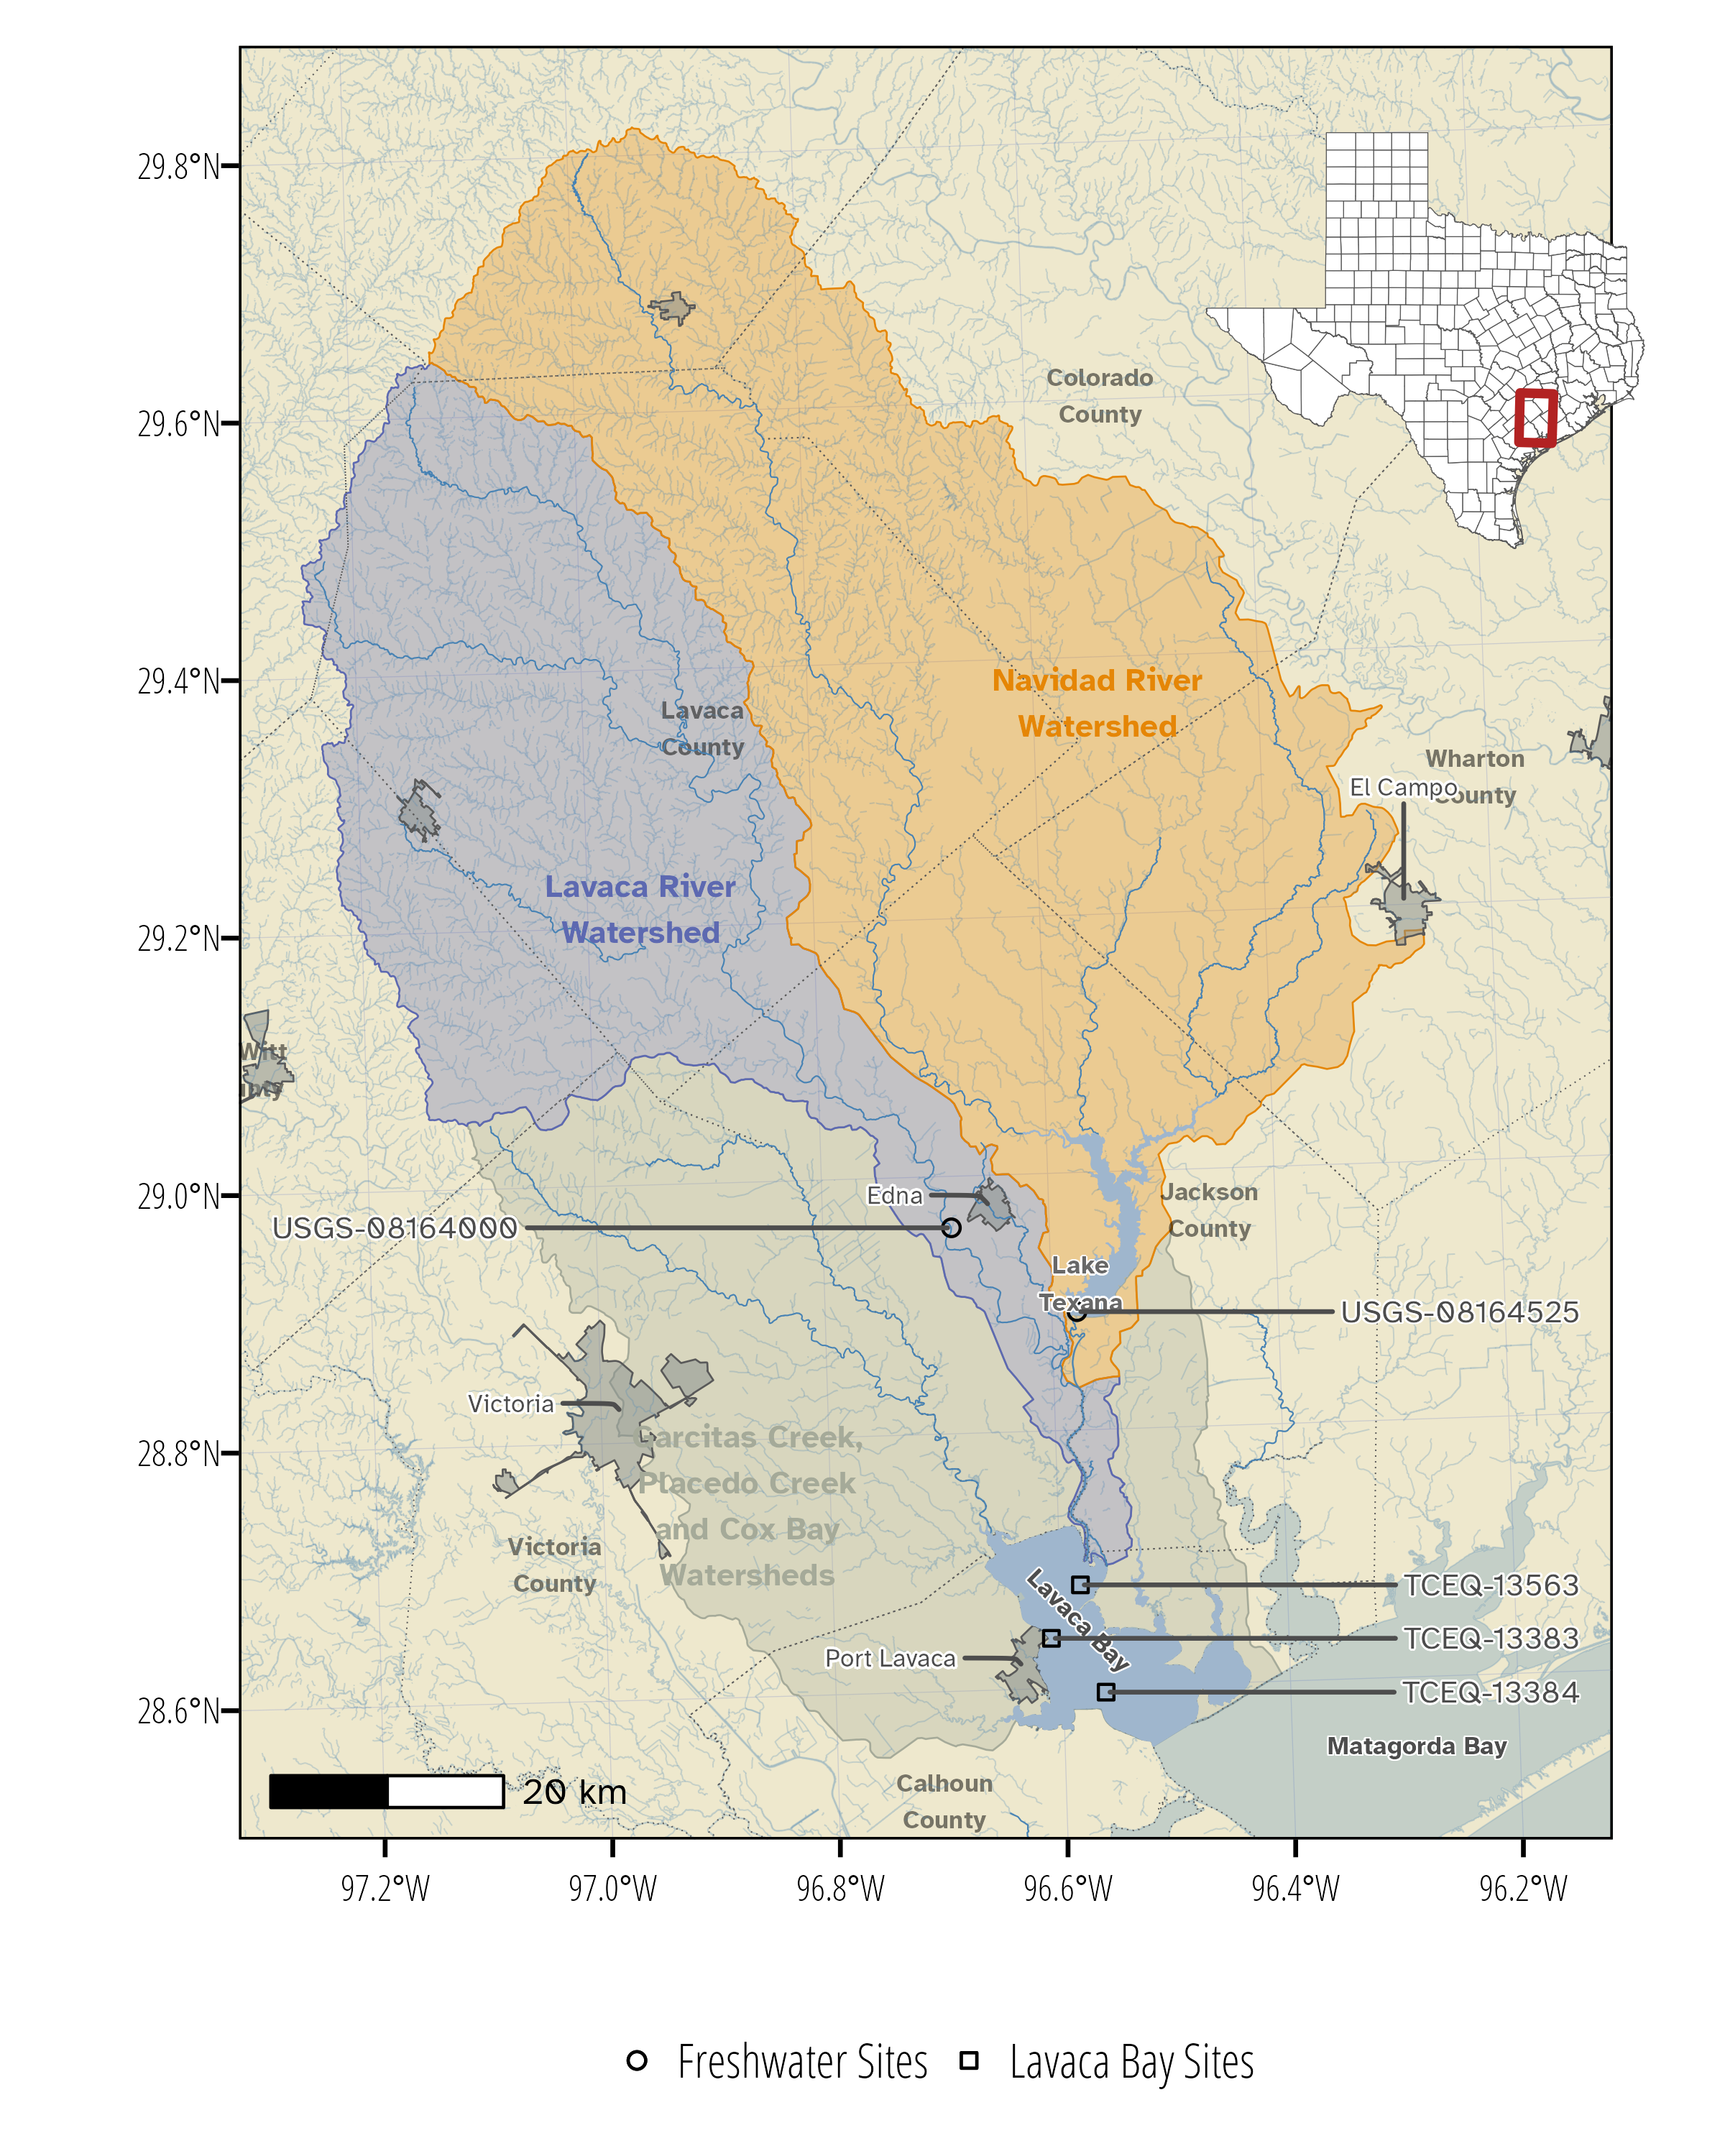
\includegraphics[width=15.5cm]{Schramm-Manuscript-2023_files/figure-latex/fig1-1.png}
\end{adjustwidth}
\caption{Map of the Lavaca Bay watershed, location of USGS gages where nutrient loads were calculated, and location of estuary water quality sampling sites.\label{fig1}}
\end{figure}

Daily discharges for the Lavaca River (USGS-08164000) were obtained from
the United States Geologic Survey (USGS) National Water Information
System using the \emph{dataRetrieval} R package
\citep{deciccoDataRetrievalPackagesDiscovering2022}. Gaged dailly
discharges from Lake Texana (USGS-0816425) were provided by the Texas
Water Development Board (TWDB) (April 21, 2022 email from R. Neupane,
TWDB).

Water quality sample data for both freshwater and estuary locations were
o btained from the Texas Commission on Environmental Quality (TCEQ)
Surface Water Quality Monitoring Information System. Data submitted
through the system are required to be collected under Quality Assurance
Project Plans and lab method procedures outlined by the TCEQ's
procedures manual. The QAPP and procedures manuals ensure the consistent
collection and laboratory methods are applied between samples collected
by different entities and under different projects. For freshwater
locations, total phosphorus (TP) and nitrate-nitrogen
(NO\textsubscript{3}) data were downloaded (Table \ref{tab:fwsummary}).
Unfortunately, insufficient data was available for assessment of total
nitrogen (TN) and total Kjeldahl nitrogen (TKN) loadings, so analysis
was restricted to TP and NO\textsubscript{3} loads. For estuary
locations, we obtained data for TP, Nitrite+Nitrate
(NO\emph{\textsubscript{x}}), TKN, chlorophyll-\emph{a}, and dissolved
oxygen (Table \ref{tab:estuarysummary}).

\begin{table}[H]

\caption{\label{tab:fwsummary}Summary of gauged streamflow and freshwater water quality samples between January 1, 2000 and December 31, 2020.}
\centering
\begin{tabular}[t]{llrrr}
\toprule
Station ID &   & Mean & SD & N\\
\midrule
USGS-08164000 & TP (mg/L) & \num{0.21} & \num{0.09} & 80\\
 & NO\textsubscript{3} (mg/L) & \num{0.18} & \num{0.24} & 74\\
 & Mean Daily Streamflow (cfs) & \num{332.78} & \num{1667.47} & 7671\\
USGS-08164525 & TP (mg/L) & \num{0.20} & \num{0.08} & 81\\
 & NO\textsubscript{3} (mg/L) & \num{0.29} & \num{0.26} & 62\\
 & Mean Daily Streamflow (cfs) & \num{666.14} & \num{2957.79} & 7671\\
\bottomrule
\end{tabular}
\end{table}

\begin{table}[H]

\caption{\label{tab:estuarysummary}Summary of estuary water quality samples collected between January 1, 2005 and December 31, 2020.}
\centering
\begin{tabular}[t]{lllll}
\toprule
Station ID &   & Mean & SD & N\\
\midrule
 & TP (mg/L) & 0.11 & 0.05 & 47\\

 & NO\textsubscript{\emph{x}} (mg/L) & 0.07 & 0.15 & 51\\

 & TKN (mg/L) & 0.94 & 0.49 & 45\\

 & Chlorophyll-\emph{a} ($\mu$g/L) & 9.43 & 5.31 & 47\\

\multirow{-5}{*}{\raggedright\arraybackslash TCEQ-13383} & DO (mg/L) & 7.22 & 1.35 & 55\\
\cmidrule{1-5}
 & TP (mg/L) & 0.08 & 0.03 & 51\\

 & NO\textsubscript{\emph{x}} (mg/L) & 0.06 & 0.08 & 52\\

 & TKN (mg/L) & 0.76 & 0.40 & 48\\

 & Chlorophyll-\emph{a} ($\mu$g/L) & 8.22 & 6.44 & 46\\

\multirow{-5}{*}{\raggedright\arraybackslash TCEQ-13384} & DO (mg/L) & 7.51 & 1.32 & 54\\
\cmidrule{1-5}
 & TP (mg/L) & 0.13 & 0.06 & 50\\

 & NO\textsubscript{\emph{x}} (mg/L) & 0.09 & 0.13 & 53\\

 & TKN (mg/L) & 0.94 & 0.37 & 49\\

 & Chlorophyll-\emph{a} ($\mu$g/L) & 9.67 & 5.33 & 49\\

\multirow{-5}{*}{\raggedright\arraybackslash TCEQ-13563} & DO (mg/L) & 7.91 & 1.34 & 56\\
\bottomrule
\end{tabular}
\end{table}

\hypertarget{estimating-watershed-based-nutrient-loads}{%
\subsection{Estimating Watershed Based Nutrient
Loads}\label{estimating-watershed-based-nutrient-loads}}

Estimates of nutrient loads were developed using Generalized Additive
Models (GAMs) relating nutrient concentration to river discharge,
season, and time. Separate models were fit at each station for each
parameter and used to predict nutrient concentrations for each day in
the study period. GAMs can be specified in a functionally similar manner
to the commonly used LOADEST \citep{cohn_validity_1992} or WRTDS
\citep{hirsch_weighted_2010} regression models and have been shown to
produce reliable estimates of nutrient and sediment loadings
\citep{wangLoadEstimationUncertainties2011, kroonRiverLoadsSuspended2012, kuhnert_quantifying_2012, robson_prediction_2015-1, hagemannEstimatingNutrientOrganic2016, mcdowell_implications_2021, biagi_novel_2022}.
GAMs are a semiparametric extension of generalized linear models where
the linear predictor is represented as the sum of multiple unknown
smooth functions and parametric linear predictors
\citep{wood_fast_2011}. Although the underlying parameter estimation
procedure of GAMs is substantially different than WRTDS, both the
functional form and results are demonstrated to be similar
\citep{beckNumericalQualitativeContrasts2017}. The use of GAMs over
other regression-based approaches was (1) the ability to easily explore
and incorporate different model terms, (2) the ability to incorporate
non-linear smooth function without explicit apriori knowledge of the
expect shape, and (3) the ability to specify a link function that
relates the expected value of the response to the linear predictors and
allows use to avoid data transformations as much as possible.

GAMs were fit using the \emph{mgcv} package in R which makes available
multiple types of smooth functions with automatic smoothness selection
\citep{wood_fast_2011}. The general form of the model relating
NO\textsubscript{3} and TP concentration to streamflow, season, and time
was:

\begin{equation}\label{eq:1}
\begin{aligned}
g(\mu) &= \alpha + f_1(ddate) + f_2(yday) + f_3(log1p(Q)) + f_4(ma) + f_5(fa)  \\
y &\sim \mathcal{N}(\mu,\,\sigma^{2}),
\end{aligned}
\end{equation}

where \(\mu\) is the conditional expected NO\textsubscript{3}-N or TP
concentration, \emph{g()} is the log-link, \(\alpha\) is the intercept,
\emph{f\textsubscript{n}()} are smoothing functions. \emph{y} is the
response variable (NO\textsubscript{3} or TP concentration) modeled as
normally distributed with mean \(\mu\) and standard deviation
\(\sigma\). \emph{ddate} is the date converted to decimal notation,
\emph{yday} is numeric day of year (1-366), and \emph{log1p(Q)} is the
natural log of mean daily streamflow plus 1.

Moving average (\emph{ma}) is an exponentially smoothed moving average
that attempts to incorporate the influence of prior streamflow events on
concentration at the current time period.
\citet{wangLoadEstimationUncertainties2011},
\citet{kuhnert_quantifying_2012} and \citet{zhang_improving_2017} refer
to this as averaged or smoothed discounted flow and demonstrated
improvements in nutrient loading models by including the term.
\citet{kuhnert_quantifying_2012} expresses MA as:

\begin{equation}\label{eq:2}
ma(\delta) = d{\kappa_{i-1}}+(1-\delta)\hat{q}_{i-1}\quad\text{and}\quad \kappa_{i}=\sum_{m=1}^{i}\hat{Q}_m,
\end{equation}

where \(\delta\) is the discount factor (here, set equal to 0.95),
\(\kappa_i\) is the cumulative flow (\emph{Q}) up to the \emph{i}th day.

Flow anomaly (\emph{fa}) is a unitless term that represents how wet or
dry the current time period is from a previous time period
\citep{vecchia_trends_2009, zhang_improving_2017}. Long-term flow
anomaly (\emph{ltfa}) is the streamflow over the previous year relative
to the entire period and calculated as described by
\citet{zhang_improving_2017}:

\begin{equation}\label{eq:3}
ltfa(t) = \bar{x}_{1\,year}(t) - \bar{x}_{entire\,period} 
\end{equation}

and the short-term flow anomaly (\emph{stfa}) calculated as the current
day flow compared to the preceding 1-month streamflow:

\begin{equation}\label{eq:4}
stfa(t) = x_{current\,day}(t) - \bar{x}_{1\,month}(t) 
\end{equation}

where \emph{x} are the averages of log-transformed streamflow over the
antecedent period (\emph{1-year}, \emph{1-month}, etc.) for time
\emph{t}. We used \emph{ltfa} in NO\textasciitilde3 models and
\emph{stfa} in TP models based on results from
\citet{zhang_improving_2017} demonstrating major improvements in
NO\textsubscript{x} regression models that incorporated \emph{ltfa} and
moderate improvements in TP regression models that incorporated
\emph{stfa}.

The calculation of model terms for the Lake Texana site were slightly
modified because daily loads are not a function of natural stream flow
processes alone, but of dam releases and nutrient concentrations at the
discharge point of the lake. \emph{Q}, \emph{ma}, and \emph{fa} terms
were calculated based on total gaged inflow from the 4 major tributaries
to the lake. Thin-plate regression splines were used for \emph{ddate},
\emph{log1p(Q)}, \emph{fa}, and \emph{ma}. A cyclic cubic regression
spline was used for \emph{yday} to ensure the ends of the spline match
(day 1 and day 366 are expected to match). First order penalties were
applied to the smooths of flow-based variables which penalize departures
from a flat function to help constrain extrapolations for high flow
measurements.

Left-censored data were not uncommon in this dataset. Several methods
are available to account for censored data. We transformed left-censored
nutrient concentrations to one-half the detection limit. Although this
simple approach can introduce bias
\citep{hornungEstimationAverageConcentration1990}, we considered it
acceptable because high concentrations and loadings are associated with
high-flow events and low-flow/low-concentration events will account for
a small proportion of total loadings \citep{mcdowell_implications_2021}.

Daily loads were estimated as the predicted concentration multiplied by
the daily streamflow. For the Lake Texana site, model terms were
slightly modified because daily loads are a function of dam releases and
nutrient concentration, but concentration will be a function of lake
inflows and or other lake processes. \emph{Q}, \emph{ma}, and \emph{fa}
terms were calculated based on total gaged inflow from the 4 major
tributaries to the lake and laily loads at the dam were calculated from
the discrete daily concentration at the discharge point of the lake and
corresponding reported daily discharge from the dam. Flow-normalized
loads were estimated similar to WRTDS by setting flow-based covariates
on each day of the year equal to each of the historical values for that
day of the year over the study period \citep{hirsch_weighted_2010}. The
flow-normalized estimate was calculated as the mean of all the
predictions for each day considering all possible flow values. Standard
deviations and credible intervals were obtained by drawing samples from
the multivariate normal posterior distribution of the fitted GAM
\citep{woodConfidenceIntervalsGeneralized2006, marraCoveragePropertiesConfidence2012, mcdowell_implications_2021}.
Uncertainty in loads were reported as 90\% credible intervals developed
by drawing 1000 realizations of parameter estimates from the
multivariate normal posterior distribution of the model parameters. GAM
performance was evaluated using repeated 5-fold cross validation
\citep{burmanComparativeStudyOrdinary1989} and average Nash-Suttclifee
Efficiency (NSE), r\textsuperscript{2} and percent bias (PBIAS) metrics
across folds were calculated for each model.

\hypertarget{linking-estuary-water-quality-to-hydrology-and-nutrient-loads}{%
\subsection{Linking Estuary Water Quality to Hydrology and Nutrient
Loads}\label{linking-estuary-water-quality-to-hydrology-and-nutrient-loads}}

To test if changes in freshwater inflow and nutrient loading had
explanatory effect on changes in estuary water quality a series of GAM
models were fit at each site relating parameter concentration to
temporal trends, inflow, and nutrient loads
\citep{murphyNutrientImprovementsChesapeake2022}:

\begin{equation}\label{eq:5}
\begin{aligned}
g(\mu) &= \alpha + f_1(ddate) + f_2(yday) \\
y &\sim \Gamma(\mu,\lambda),
\end{aligned}
\end{equation}

\begin{equation}\label{eq:6}
\begin{aligned}
g(\mu) &= \alpha + f_1(ddate) + f_2(yday) + f_3(Q) \\
y &\sim \Gamma(\mu,\lambda),
\end{aligned}
\end{equation}

\begin{equation}\label{eq:7}
\begin{aligned}
g(\mu) &= \alpha + f_1(ddate) + f_2(yday) + f_3(Q) + f_4(Load) \\
y &\sim \Gamma(\mu,\lambda),
\end{aligned}
\end{equation}

where \(\mu\) is the conditional expected response (nutrient
concentration), \emph{g()} is the log link, and response variable was
modeled as Gamma distributed with mean \(\mu\) and scale \(\lambda\).
\emph{f\textsubscript{1}(ddate)} is decimal date smoothed with a
thin-plate regression spline, \emph{f\textsubscript{2}(yday)} is the
numeric day of year smoothed with a cyclic cubic regression spline,
\emph{f\textsubscript{3}(Q)} is mean daily inflow (the combined
measurements from Lavaca River and Lake Texana) and
\emph{f\textsubscript{4}(Load)} is the total NO\textsubscript{3} or TP
watershed load. The set of models specified for each water quality
response are in Table \ref{rab:estgammodels}.

\begin{table}[H]

\caption{\label{tab:estgammodels}Set of GAM models specified for each water quality parameter response.}
\centering
\begin{tabular}[t]{lll}
\toprule
\makecell[l]{Water Quality\\Response Parameter} & Model & Model Terms\\
\midrule
 & Temporal & s(ddate) + s(yday)\\

 & Flow & s(ddate) + s(yday) + s(Q)\\

\multirow{-3}{*}{\raggedright\arraybackslash TP} & Flow+Load & s(ddate) + s(yday) + s(Q) + s(TP Load)\\
\cmidrule{1-3}
 & Temporal & s(ddate) + s(yday)\\

 & Flow & s(ddate) + s(yday) + s(Q)\\

\multirow{-3}{*}{\raggedright\arraybackslash NO\textsubscript{\emph{x}}} & Flow+Load & s(ddate) + s(yday) + s(Q) + s(NO\textsubscript{3} Load)\\
\cmidrule{1-3}
 & Temporal & s(ddate) + s(yday)\\

 & Flow & s(ddate) + s(yday) + s(Q)\\

\multirow{-3}{*}{\raggedright\arraybackslash Chlorophyll-\emph{a}} & Flow+Load & s(ddate) + s(yday) + s(Q) + s(TP Load) + s(NO\textsubscript{3} Load)\\
\cmidrule{1-3}
 & Temporal & s(ddate) + s(yday)\\

 & Flow & s(ddate) + s(yday) + s(Q)\\

\multirow{-3}{*}{\raggedright\arraybackslash Dissolved Oxygen} & Flow+Load & s(ddate) + s(yday) + s(Q) + s(TP Load) + s(NO\textsubscript{3}  Load)\\
\cmidrule{1-3}
 & Temporal & s(ddate) + s(yday)\\

\multirow{-2}{*}{\raggedright\arraybackslash TKN} & Flow & s(ddate) + s(yday) + s(Q)\\
\bottomrule
\end{tabular}
\end{table}

Because streamflow and nutrient loads are tightly correlated, freshwater
inflow masks any potential signals from nutrient loads alone. Following
the methodology implemented by
\citet{murphyNutrientImprovementsChesapeake2022}, both streamflow and
nutrient loads were prepossessed to account for season and flow. Instead
of using raw freshwater inflow and nutrient loading values, these values
were replaced by seasonally adjusted inflow and flow-adjusted nutrient
loads by fitting a GAM relating season (day of year) to log transformed
daily freshwater inflow values:

\begin{equation}\label{eq:8}
g(\mu) = \alpha + f_1(yday),
\end{equation}

and a GAM relating log transformed NO\textsubscript{3} or TP loads to
log transformed daily inflow:

\begin{equation}\label{eq:9}
g(\mu) = \alpha + f_1(log(Q)),
\end{equation}

where the response variables were modeled as normally distributed with
an identity link function. Response residuals from the respective GAM
models were used as \emph{Q} and \emph{Load} in Equation \ref{eq:6} and
Equation \ref{eq:7}.

\hypertarget{results}{%
\section{Results}\label{results}}

\hypertarget{watershed-nutrient-loads}{%
\subsection{Watershed Nutrient Loads}\label{watershed-nutrient-loads}}

Lavaca NO\textsubscript{3} r2 = 0.85 and 0.90 deviance explained TP r2 =
0.27 and 0.33 Texana NO\textsubscript{3} r2 = 0.75 and 0.81 TP = 0.32
and 0.38

\begin{figure}
\centering
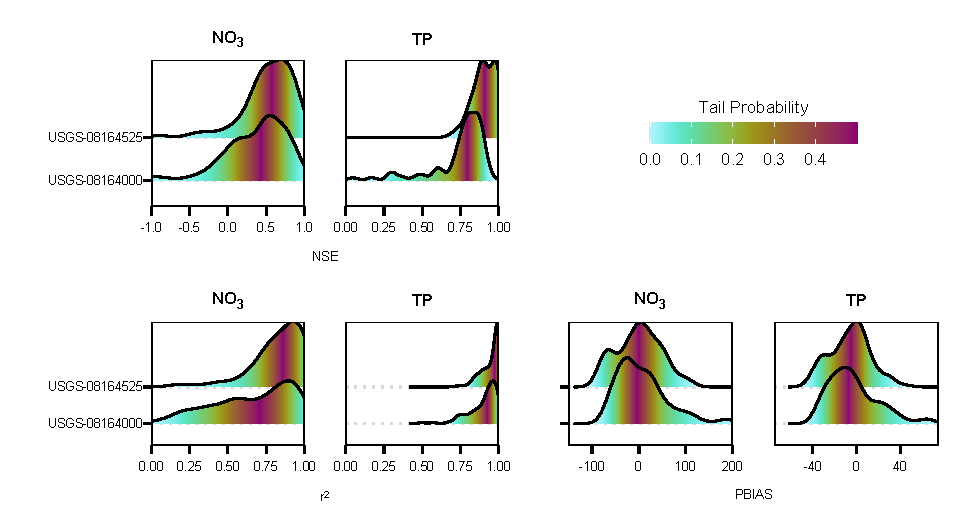
\includegraphics{Schramm-Manuscript-2023_files/figure-latex/fig2-1.pdf}
\caption{Density plots of goodness-of-fit metrics from repeated 5-fold
cross validation. Color indicates the tail probability calcualted from
the empirical cumulative distribution of the goodness-of-fit metrics.}
\end{figure}

\begin{figure}
\centering
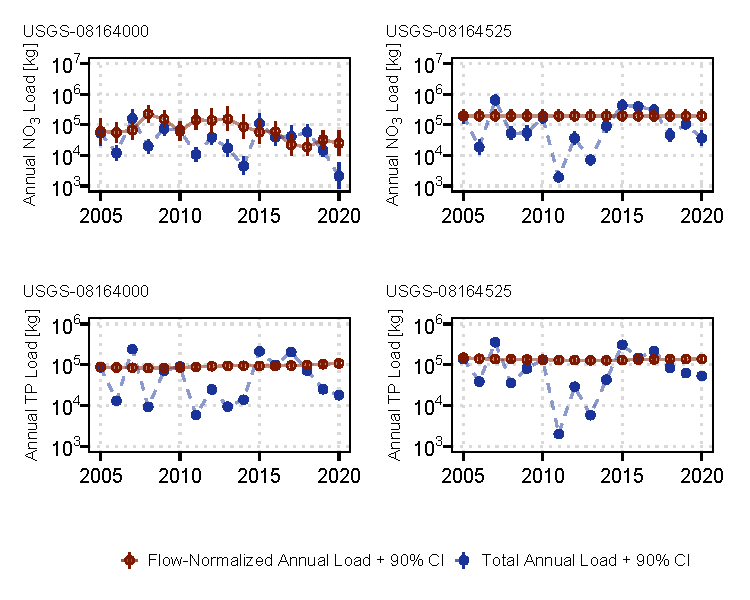
\includegraphics{Schramm-Manuscript-2023_files/figure-latex/fig3-1.pdf}
\caption{Aggregated estimated annual and flow-normalized annual
NO\textsubscript{3} and TP loads for USGS-08164000 and USGS-08164525.}
\end{figure}

\begin{figure}
\centering
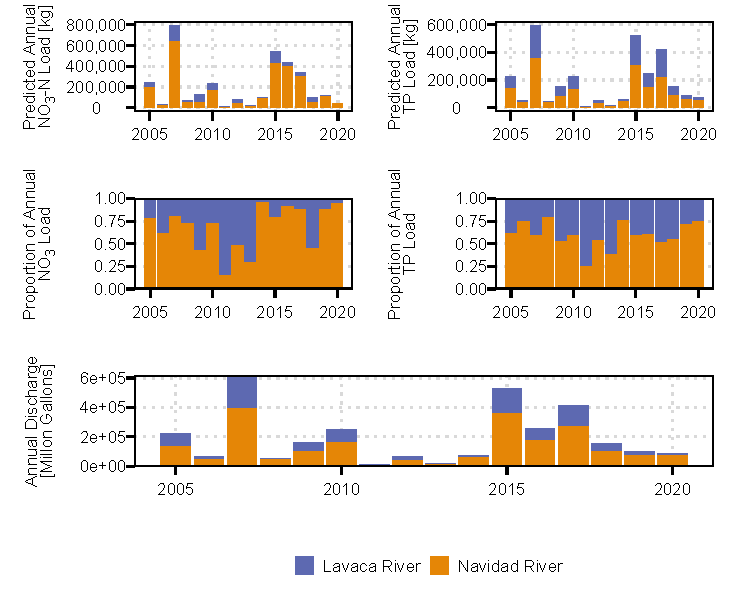
\includegraphics{Schramm-Manuscript-2023_files/figure-latex/fig4-1.pdf}
\caption{Comparison of delivered annual loads at USGS-08164000 and
USGS-08164525.}
\end{figure}

\hypertarget{linkages-between-water-quality-and-watershed-flows-and-loads}{%
\subsection{Linkages Between Water Quality and Watershed Flows and
Loads}\label{linkages-between-water-quality-and-watershed-flows-and-loads}}

\begin{verbatim}
## Usually it is recommended to use column_spec before collapse_rows, especially in LaTeX, to get a desired result. 
## Usually it is recommended to use column_spec before collapse_rows, especially in LaTeX, to get a desired result. 
## Usually it is recommended to use column_spec before collapse_rows, especially in LaTeX, to get a desired result.
\end{verbatim}

\begin{table}[H]

\caption{\label{tab:unnamed-chunk-1}Model AIC\textsubscript{c} values and associated model probabilities (in parenthesis). Models with the highest probability for each site and water quality parameter combination are bolded and italicized for emphasis.}
\centering
\begin{tabular}[t]{ll>{}l>{}l>{}l}
\toprule
Parameter & Site & Temporal & Flow & Flow + Load\\
\midrule
 & TCEQ-13383 & -152.1 (0.03) & -156.1 (0.24) & \em{\textbf{-158.2 (0.72)}}\\

 & TCEQ-13384 & -194.4 (0.03) & \em{\textbf{-200.2 (0.49)}} & -200.2 (0.49)\\

\multirow{-3}{*}{\raggedright\arraybackslash TP} & TCEQ-13563 & -145.3 (0) & -156.6 (0.41) & \em{\textbf{-157.3 (0.59)}}\\
\cmidrule{1-5}
 & TCEQ-13383 & -218.9 (0) & \em{\textbf{-244.8 (0.5)}} & -244.8 (0.5)\\

 & TCEQ-13384 & -263.4 (0) & -311.7 (0.48) & \em{\textbf{-311.9 (0.52)}}\\

\multirow{-3}{*}{\raggedright\arraybackslash NO\textsubscript{\emph{x}}} & TCEQ-13563 & -175.1 (0) & \em{\textbf{-190.2 (0.5)}} & -190.2 (0.5)\\
\cmidrule{1-5}
 & TCEQ-13383 & 279.7 (0.18) & \em{\textbf{278.1 (0.41)}} & 278.1 (0.41)\\

 & TCEQ-13384 & \em{\textbf{268.2 (0.33)}} & 268.2 (0.33) & 268.2 (0.33)\\

\multirow{-3}{*}{\raggedright\arraybackslash Chlorophyll-\emph{a}} & TCEQ-13563 & 289.5 (0.08) & \em{\textbf{286.1 (0.46)}} & 286.1 (0.46)\\
\cmidrule{1-5}
 & TCEQ-13383 & \em{\textbf{42.2 (0.66)}} & 43.5 (0.34) & -\\

 & TCEQ-13384 & \em{\textbf{34.3 (0.57)}} & 34.8 (0.43) & -\\

\multirow{-3}{*}{\raggedright\arraybackslash TKN} & TCEQ-13563 & 31.1 (0.22) & \em{\textbf{28.7 (0.78)}} & -\\
\cmidrule{1-5}
 & TCEQ-13383 & \em{\textbf{146.4 (0.34)}} & 146.4 (0.34) & 146.5 (0.32)\\

 & TCEQ-13384 & \em{\textbf{135.9 (0.47)}} & 137 (0.27) & 137 (0.27)\\

\multirow{-3}{*}{\raggedright\arraybackslash DO} & TCEQ-13563 & 138.3 (0.25) & \em{\textbf{137.2 (0.43)}} & 137.8 (0.32)\\
\bottomrule
\end{tabular}
\end{table}

\hypertarget{figures-tables-and-schemes}{%
\subsection{Figures, Tables and
Schemes}\label{figures-tables-and-schemes}}

\hypertarget{formatting-of-mathematical-components}{%
\subsection{Formatting of Mathematical
Components}\label{formatting-of-mathematical-components}}

This is an example of an equation:

\begin{equation}
a = 1,
\end{equation}

the text following an equation need not be a new paragraph. Please
punctuate equations as regular text.

This is the example 2 of equation:

\begin{adjustwidth}{-\extralength}{0cm}
\begin{equation}
a = b + c + d + e + f + g + h + i + j + k + l + m + n + o + p + q + r + s + t + 
u + v + w + x + y + z
\end{equation}
\end{adjustwidth}

\hypertarget{discussion}{%
\section{Discussion}\label{discussion}}

\begin{table}[H]

\begin{tabular}[t]{lllll}
\toprule
Parameter & \makecell[c]{Reported Yield\\(kg$\cdot$km\textsuperscript{-2}$\cdot$year\textsuperscript{-1})} & Approach & Time Period & Reference\\
\midrule
TP & 42.9 (34.4, 54.0) & GAM & 2000-2020 & -\\
TP & 45.2 & SPARROW & 2012 & @wiseSpatiallyReferencedModels2019\\
TP & 42 & SWAT & 1977-2005 & @omaniEstimationSedimentNutrient2014\\
TP & 20.81-91.58 & SPARROW & 2002 & @rebichSourcesDeliveryNutrients2011\\
TP & 28.9 & LOADEST & 1972-1993 & @dunnTrendsNutrientInflows1996\\
\bottomrule
\end{tabular}
\end{table}

Authors should discuss the results and how they can be interpreted in
perspective of previous studies and of the working hypotheses. The
findings and their implications should be discussed in the broadest
context possible. Future research directions may also be highlighted.

\hypertarget{conclusion}{%
\section{Conclusion}\label{conclusion}}

This section is not mandatory, but can be added to the manuscript if the
discussion is unusually long or complex.

%%%%%%%%%%%%%%%%%%%%%%%%%%%%%%%%%%%%%%%%%%

\vspace{6pt}

%%%%%%%%%%%%%%%%%%%%%%%%%%%%%%%%%%%%%%%%%%
%% optional

% Only for the journal Methods and Protocols:
% If you wish to submit a video article, please do so with any other supplementary material.
% \supplementary{The following supporting information can be downloaded at: \linksupplementary{s1}, Figure S1: title; Table S1: title; Video S1: title. A supporting video article is available at doi: link.}

%%%%%%%%%%%%%%%%%%%%%%%%%%%%%%%%%%%%%%%%%%

\funding{This paper was funded by financial assistance provided by the
Coastal Zone Management Act of 1972, as amended, administered by the
National Oceanic and Atmospheric Administration (NOAA), Office for
Coastal Management, pursuant to NOAA Award No.~NA21NOS4190136. The views
expressed herein are those of the author(s) and do not necessarily
reflect the views of NOAA, the U.S. Department of Commerce, or any of
their subagencies.}



\dataavailability{Data and code are openly available in Zenodo at
\url{https://doi.org/10.5281/zenodo.7330754}.}

\acknowledgments{All sources of funding of the study should be
disclosed. Please clearly indicate grants that you have received in
support of your research work. Clearly state if you received funds for
covering the costs to publish in open access.}

\conflictsofinterest{The author declares no conflict of interest. The
founding sponsors had no role in the design of the study; in the
collection, analyses, or interpretation of data; in the writing of the
manuscript, an in the decision to publish the results.}

%%%%%%%%%%%%%%%%%%%%%%%%%%%%%%%%%%%%%%%%%%
%% Optional

%% Only for journal Encyclopedia
%\entrylink{The Link to this entry published on the encyclopedia platform.}


%%%%%%%%%%%%%%%%%%%%%%%%%%%%%%%%%%%%%%%%%%
%% Optional
%%%%%%%%%%%%%%%%%%%%%%%%%%%%%%%%%%%%%%%%%%
\begin{adjustwidth}{-\extralength}{0cm}

%\printendnotes[custom] % Un-comment to print a list of endnotes


\reftitle{References}

% Please provide either the correct journal abbreviation (e.g. according to the “List of Title Word Abbreviations” http://www.issn.org/services/online-services/access-to-the-ltwa/) or the full name of the journal.
% Citations and References in Supplementary files are permitted provided that they also appear in the reference list here.

%=====================================
% References, variant A: external bibliography
%=====================================
\externalbibliography{yes}
\bibliography{mybibfile.bib}

% If authors have biography, please use the format below
%\section*{Short Biography of Authors}
%\bio
%{\raisebox{-0.35cm}{\includegraphics[width=3.5cm,height=5.3cm,clip,keepaspectratio]{Definitions/author1.pdf}}}
%{\textbf{Firstname Lastname} Biography of first author}
%
%\bio
%{\raisebox{-0.35cm}{\includegraphics[width=3.5cm,height=5.3cm,clip,keepaspectratio]{Definitions/author2.jpg}}}
%{\textbf{Firstname Lastname} Biography of second author}

% For the MDPI journals use author-date citation, please follow the formatting guidelines on http://www.mdpi.com/authors/references
% To cite two works by the same author: \citeauthor{ref-journal-1a} (\citeyear{ref-journal-1a}, \citeyear{ref-journal-1b}). This produces: Whittaker (1967, 1975)
% To cite two works by the same author with specific pages: \citeauthor{ref-journal-3a} (\citeyear{ref-journal-3a}, p. 328; \citeyear{ref-journal-3b}, p.475). This produces: Wong (1999, p. 328; 2000, p. 475)

%%%%%%%%%%%%%%%%%%%%%%%%%%%%%%%%%%%%%%%%%%
%% for journal Sci
%\reviewreports{\\
%Reviewer 1 comments and authors’ response\\
%Reviewer 2 comments and authors’ response\\
%Reviewer 3 comments and authors’ response
%}
%%%%%%%%%%%%%%%%%%%%%%%%%%%%%%%%%%%%%%%%%%
\PublishersNote{}
\end{adjustwidth}


\end{document}
